\documentclass[a4paper,12pt]{article}
\usepackage[utf8]{inputenc}
\usepackage{geometry}
\geometry{
 a4paper,
 left=1.25in,
 right=1.25in,
 top=1in,
 }
\usepackage[croatian,english]{babel}    %za hrvatske naslove
\usepackage[nottoc]{tocbibind}  %za pravilan table of content
\usepackage{graphicx}   %za dodavanje slika
\usepackage{amsmath}    %za matematičke forumele
\usepackage{subcaption} %za dvije slike u jednoj
\usepackage{booktabs}   %za bolje tablice
\usepackage{cite}

\begin{document}

\begin{center}
SVEUČILIŠTE JURJA DOBRILE U PULI 

FAKULTET INFORMATIKE

\vspace{45mm} 

\textbf{Ime Prezime}

\vspace{20mm} 

\textbf{Naslov rad}

\vspace{5mm}
DIPLOMSKI/ZAVRSNI RAD

\vfill

%Upisat tocan mjesec i godinu
Pula, rujan, 2025. godine
\end{center}

\pagenumbering{gobble}
\clearpage
\newpage

\begin{center}
SVEUČILIŠTE JURJA DOBRILE U PULI 

FAKULTET INFORMATIKE

\vspace{45mm} 

\textbf{Neven Nižić}

\vspace{20mm} 

\textbf{"Optimizacija raspodjele projektnih aktivnosti primjenom genetskih algoritama i Monte Carlo simulacije"}

\vspace{5mm}
DIPLOMSKI RAD

\end{center}

\vspace{45mm}

\textbf{JMBAG: 0303118917, izvanredni student}

\textbf{Studijski smjer: Informatika}
\bigskip

\textbf{Kolegij: Modeliranje i simulacije}

\textbf{Znanstveno područje : Društvene znanosti}

\textbf{Znanstveno polje : Informacijske i komunikacijske znanosti}

\textbf{Znanstvena grana : Informacijski sustavi i informatologija}
\bigskip

\textbf{Mentor: dr.sc. Darko Etinger}

\vfill

\begin{center}

%Upisat tocan mjesec i godinu
Pula, rujan, 2025. godine

\end{center}

\pagenumbering{gobble}
\clearpage
\newpage

%Resetirat margine
\restoregeometry

\selectlanguage{croatian}
\begin{abstract}
Upravljanje projektima često uključuje složene odluke vezane uz raspodjelu aktivnosti i resursa, osobito u uvjetima nesigurnosti i vremenskih ograničenja. Tradicionalne metode kao što su PERT i CPM često ne uspijevaju obuhvatiti stohastičku prirodu stvarnih projekata. U ovom radu razvijen je i evaluiran hibridni optimizacijski pristup temeljen na genetskim algoritmima (GA) i Monte Carlo (MC) simulaciji. Kroz dvo-fazni eksperimentalni dizajn, provedena je sustavna usporedba tri modela: nasumične pretrage, jedno-kriterijskog GA usmjerenog isključivo na povrat na investiciju (ROI), te više-kriterijskog GA+MC modela (NSGA-II) koji istovremeno optimizira ROI i rizik trajanja projekta. Rezultati dobiveni na sintetičkim podacima različite složenosti i restriktivnosti pokazuju da, iako jedno-kriterijski GA najučinkovitije maksimizira profit, hibridni GA+MC model uspješno generira Paretov front rješenja koja nude optimalan kompromis između profitabilnosti i trajanja. Nadalje, istraživanje je otkrilo ključan nalaz: pod ekstremno restriktivnim budžetom, robusnost jednostavnijeg, jedno-kriterijskog GA nadmašuje onu složenijeg, više-kriterijskog modela. Rad zaključuje da ne postoji univerzalno superioran model, već da optimalan izbor ovisi o strateškim prioritetima – maksimizaciji profita naspram uravnoteženog upravljanja rizikom.
\end{abstract}
\begin{small}
\textbf{Ključne riječi:} projektno upravljanje, genetski algoritam, Monte Carlo simulacija, više-kriterijska optimizacija, upravljanje rizikom, Paretov front, NSGA-II
\end{small}

\bigskip

\selectlanguage{english}
\begin{abstract}
Project management often involves complex decisions regarding the allocation of activities and resources, especially under conditions of uncertainty and constraints. Traditional methods such as PERT and CPM frequently fail to capture the stochastic nature of real-world projects. This thesis develops and evaluates a hybrid optimization approach based on genetic algorithms (GA) and Monte Carlo (MC) simulation. Through a two-phase experimental design, a systematic comparison of three models was conducted: random search, a single-objective GA focused solely on return on investment (ROI), and a multi-objective GA+MC model (NSGA-II) that simultaneously optimizes ROI and project duration risk. The results, obtained from synthetic data of varying complexity and restrictiveness, show that while the single-objective GA is most effective at maximizing profit, the hybrid GA+MC model successfully generates a Pareto front of solutions offering an optimal trade-off between profitability and duration. Furthermore, the research revealed a key finding: under extremely restrictive budget constraints, the robustness of the simpler, single-objective GA surpasses that of the more complex, multi-objective model. The thesis concludes that there is no universally superior model; rather, the optimal choice depends on strategic priorities—maximizing profit versus balanced risk management.
\end{abstract}
\begin{small}
\textbf{Keywords:} project management, genetic algorithm, Monte Carlo simulation, multi-objective optimization, risk management, Pareto front, NSGA-II
\end{small}

\pagenumbering{gobble}
\clearpage
\newpage

\selectlanguage{croatian}
\tableofcontents
\pagenumbering{gobble}
\clearpage
\newpage

\pagenumbering{arabic}

\section{Uvod}

Upravljanje projektima obuhvaća niz izazova, osobito kada je riječ o optimizaciji raspodjele ograničenih resursa među konkurentskim aktivnostima. Projektni menadžeri često se suočavaju s neizvjesnostima vezanima uz trajanje zadataka, dostupnost resursa i dinamičnost okruženja. Upravo te nesigurnosti zahtijevaju robusne metode koje mogu osigurati učinkovitu alokaciju resursa unatoč stohastičkoj prirodi ulaznih podataka.

\subsection{Motivacija}

Jedan od ključnih problema u upravljanju projektima je kako rasporediti ograničene resurse (vremenske, ljudske, financijske) na skup aktivnosti tako da se minimizira ukupno trajanje projekta ili maksimizira ukupna vrijednost. Klasične determinističke metode često zanemaruju nesigurnosti koje su prisutne u stvarnim projektima, što dovodi do planova koji su nerealni i teško provedivi \cite{Kerzner2017, PMI2021}. Stoga raste interes za primjenom heurističkih i stohastičkih metoda u projektnoj optimizaciji.

\subsection{Rizici i nesigurnosti u projektnom upravljanju}

Neizvjesnost u trajanju aktivnosti, nepredviđeni događaji, promjene prioriteta i ograničeni resursi stvaraju kompleksno i promjenjivo okruženje. Klasifikacija rizika i kvantifikacija njihove vjerojatnosti ključni su za izradu kvalitetnog plana. Zbog toga se uvode stohastičke metode kao što su Monte Carlo simulacija, koje omogućuju analizu različitih scenarija i procjenu vjerojatnosti uspjeha projekta \cite{Vose2008}. Upravo zbog tih izazova, mnogi autori predlažu uporabu kvantitativnih metoda kao što su Monte Carlo simulacije za procjenu vjerojatnih vremenskih i troškovnih odstupanja \cite{Avlijas2008}.

\subsection{Heuristički pristup optimizaciji upravljanja projektima korištenjem kombiniranog stohastičkog modela}

U ovom radu predlaže se heuristički pristup optimizaciji upravljanja projektima korištenjem kombiniranog stohastičkog modela. Pritom se kombiniraju dva komplementarna pristupa:

\begin{itemize}
    \item \textbf{Genetski algoritam (GA)} – koristi se za pronalaženje optimalne ili blizu optimalne raspodjele projektnih aktivnosti, uzimajući u obzir njihovu važnost i vremenska ograničenja. GA su pokazali visoku učinkovitost kod NP-teških problema poput problema ruksaka \cite{Goldberg1989, Mitchell1998}.
    \item \textbf{Monte Carlo simulacija (MCS)} – koristi se za modeliranje neizvjesnosti u trajanju aktivnosti, često koristeći trokutastu distribuciju, posebno kada nije dostupna pouzdana povijesna statistika \cite{Law2015}.
\end{itemize}

Ova kombinacija omogućuje istraživanje velikog prostora rješenja, pri čemu se u svakoj iteraciji genetskog algoritma evaluira kvaliteta rješenja putem više Monte Carlo simulacija. Time se dobiva robusnije rješenje koje bolje odražava nesigurnost u ulaznim podacima.

\subsection{Cilj rada}

Cilj ovog rada je razviti model koji integrira genetski algoritam i Monte Carlo simulaciju u svrhu optimizacije raspodjele projektnih aktivnosti pod uvjetima nesigurnosti. Model se temelji na knapsack formulaciji problema, gdje se svaka aktivnost karakterizira očekivanim trajanjem, varijabilnošću i vrijednošću. Kroz eksperimente će se testirati učinkovitost predloženog pristupa te usporediti dobivena rješenja u kontekstu robustnosti i izvedivosti plana projekta.


Upravljanje projektima je ključna aktivnost u brojnim industrijama, od građevine i IT-a do farmaceutike i financija. Jedan od najzahtjevnijih aspekata upravljanja projektima jest učinkovita raspodjela aktivnosti i resursa kroz vrijeme, pri čemu se mora zadovoljiti niz ograničenja, uključujući budžet, vremenski rok, kapacitete resursa i međusobne ovisnosti između zadataka. U složenim projektima s velikim brojem aktivnosti, tradicionalni pristupi često nisu dostatni jer ne uspijevaju adresirati neizvjesnosti i varijabilnost koje prate realne projekte.

\subsection{Motivacija}

Raspodjela projektnih aktivnosti i resursa u uvjetima nesigurnosti i ograničenja predstavlja NP-težak problem, što znači da se broj mogućih kombinacija rješenja eksponencijalno povećava s veličinom problema. Tradicionalne metode kao što su CPM (Critical Path Method) i PERT (Program Evaluation and Review Technique) podrazumijevaju determinističke vremenske procjene i ne uključuju varijabilnost stvarnih uvjeta, što može dovesti do suboptimalnih ili čak neizvedivih planova.

Potreba za metodama koje mogu obuhvatiti stohastičku prirodu trajanja aktivnosti, dinamiku projektnog okruženja i složene međusobne odnose među aktivnostima, motivira primjenu naprednih optimizacijskih i simulacijskih tehnika.

\subsection{Rizici i nesigurnosti u projektnom upravljanju}

U stvarnim projektima, trajanja aktivnosti često nisu poznata unaprijed s potpunom sigurnošću. Kašnjenja, nedostatak resursa, promjene u specifikacijama ili nepredviđene okolnosti mogu značajno utjecati na tijek projekta. Zbog toga je važno uključiti kvantitativne metode za procjenu rizika i analizu nesigurnosti. Upravo tu se Monte Carlo simulacija ističe kao snažan alat koji omogućuje evaluaciju raspodjele mogućih ishoda i procjenu vjerojatnosti završetka projekta unutar zadanih rokova.

\subsection{Monte Carlo simulacija i genetski algoritmi}

Monte Carlo simulacija koristi slučajne uzorke za kvantificiranje nesigurnosti u modelima i omogućuje realističnije procjene vremenskih i troškovnih distribucija. U kontekstu projektnog upravljanja, ova metoda može simulirati tisuće mogućih scenarija izvedbe aktivnosti na temelju probabilističkih ulaza (npr. optimističnog, realnog i pesimističnog trajanja).

Genetski algoritmi (GA) predstavljaju jednu od najčešće korištenih metaheurističkih metoda za rješavanje složenih problema optimizacije. Temelje se na principima evolucije i prirodne selekcije te su učinkoviti u pretraživanju velikih prostora rješenja, što ih čini pogodnima za optimizaciju projektnih rasporeda.

\subsection{Cilj rada}

Cilj ovog rada je razviti model koji kombinira genetski algoritam s Monte Carlo simulacijom radi dobivanja robusnog plana raspodjele aktivnosti u projektu. Kombinacija ovih dviju metoda omogućava simultano:
\begin{itemize}
    \item optimiziranje projektnih rasporeda u uvjetima složenih ograničenja,
    \item kvantifikaciju rizika i nesigurnosti u izvedbi projekta,
    \item donošenje boljih odluka u upravljanju resursima.
\end{itemize}

Predloženi pristup testira se na simuliranim podacima i evaluira s obzirom na pouzdanost završetka projekta unutar vremenskog roka i efikasnost raspodjele resursa.


\newpage


\section{Teorijska podloga}

Ovo poglavlje pruža pregled temeljnih teorijskih koncepata ključnih za razumijevanje predloženog modela optimizacije projektnih aktivnosti. Detaljno će se objasniti Problem ruksaka kao osnova za formulaciju problema raspodjele resursa, Genetski algoritmi kao optimizacijska metaheuristika, te Monte Carlo simulacija i PERT metoda kao alati za modeliranje i analizu nesigurnosti u projektnom upravljanju.

\subsection{Knapsack problem}

Problem ruksaka (engl. \textit{Knapsack Problem}) jedan je od najpoznatijih i najčešće proučavanih problema kombinatorne optimizacije, svrstan u klasu NP-teških problema \cite{Goldberg1989}. U osnovnoj verziji, cilj je odabrati podskup objekata s pridruženom težinom i vrijednošću, s ciljem maksimiziranja ukupne vrijednosti odabranih objekata, pri čemu njihova ukupna težina ne smije prelaziti zadani kapacitet ruksaka.

Formalno, za skup od $n$ objekata, gdje svaki objekt $i$ ima težinu $w_i$ i vrijednost $v_i$, te uz zadani kapacitet ruksaka $W$, cilj je maksimizirati funkciju:

\[
\max \sum_{i=1}^n v_i x_i \quad \text{uz ograničenje} \quad \sum_{i=1}^n w_i x_i \leq W,\ x_i \in \{0,1\}
\]
gdje je $x_i = 1$ ako je objekt $i$ odabran, a $x_i = 0$ ako nije.

U kontekstu upravljanja projektima, ovaj se problem često pojavljuje u složenijim varijantama, poput višedimenzionalnog problema ruksaka (Multi-Dimensional Knapsack Problem – MDKP). U MDKP-u, osim jedne težine, svaki objekt (projektna aktivnost) ima više dimenzija "težine" koje predstavljaju različite vrste resursa (npr. vrijeme, budžet, broj radnika, specifična oprema). Kapacitet ruksaka tada predstavlja ograničenja za svaku od tih dimenzija. Projektne aktivnosti se mogu interpretirati kao objekti s određenim trajanjem, troškom i vrijednošću (npr. strateška važnost, povrat investicije – ROI), dok resursi projekta predstavljaju kapacitet ruksaka. MDKP se stoga koristi za optimalnu raspodjelu ograničenih, višestrukih resursa među konkurentskim projektnim aktivnostima, s ciljem maksimiziranja ukupne vrijednosti ili minimiziranja ukupnog trajanja projekta.

\subsection{Genetski algoritmi}

Genetski algoritmi (GA) su moćne metaheurističke optimizacijske metode inspirirane procesima prirodne selekcije i evolucije \cite{Goldberg1989, Mitchell1998}. Pripadaju široj klasi evolucijskih algoritama i iznimno su učinkoviti u rješavanju složenih optimizacijskih problema s velikim i nepreglednim prostorom rješenja, posebno onih NP-teških, za koje klasične metode nisu praktične \cite{Gandomi2013, Kaveh2012}.

Osnovni princip GA leži u simulaciji evolucije populacije potencijalnih rješenja. Svako rješenje problema kodira se kao \textit{kromosom} (obično binarni niz, ali može biti i cijeli broj, realni broj ili permutacija), a populacija kromosoma se iterativno poboljšava kroz generacije primjenom genetskih operatora. Tipični koraci genetskog algoritma uključuju:

\begin{enumerate}
    \item \textbf{Inicijalizacija populacije:} Generira se početni skup nasumičnih ili heuristički generiranih kromosoma.
    \item \textbf{Evaluacija funkcije cilja (fitness):} Svakom kromosomu dodjeljuje se vrijednost \textit{fitnessa} koja odražava kvalitetu rješenja. U kontekstu ovog rada, fitness funkcija uključuje rezultate Monte Carlo simulacije kako bi se procijenila robusnost i vjerojatnost uspjeha projekta \cite{Gandomi2013}.
    \item \textbf{Selekcija roditelja:} Kromosomi s višim fitnessom imaju veću vjerojatnost da budu odabrani kao roditelji (npr. turnirska selekcija, rulet, rang-selekcija).
    \item \textbf{Križanje (crossover):} Dva odabrana roditelja kombiniraju se kako bi se stvorili novi potomci, prenoseći genetski materijal. Ovo omogućuje istraživanje novih dijelova prostora rješenja.
    \item \textbf{Mutacija:} Slučajne, male promjene unose se u kromosome potomaka kako bi se održala genetska raznolikost populacije i izbjegla prerana konvergencija.
    \item \textbf{Zamjena populacije:} Nova generacija potomaka zamjenjuje dio ili cijelu staru populaciju, i proces se ponavlja dok se ne ispuni kriterij zaustavljanja.
\end{enumerate}

Kodiranje rješenja u problemima raspodjele projektnih aktivnosti često uključuje binarno kodiranje (gdje svaki bit predstavlja odabir ili ne-odabir aktivnosti) ili cjelobrojno kodiranje (gdje brojevi predstavljaju redoslijed aktivnosti ili dodjelu resursa). GA su posebno prikladni za probleme gdje nije poznata funkcija gradijenta, što ih čini fleksibilnima za širok spektar primjena.

\subsection{Monte Carlo simulacija}

Monte Carlo simulacija (MCS) je računska metoda koja koristi nasumično uzorkovanje za procjenu ponašanja složenog sustava ili procesa, posebno kada je analitičko rješenje teško ili nemoguće. Njena je primarna prednost sposobnost modeliranja nesigurnosti i rizika u sustavima s probabilističkim ulaznim varijablama \cite{Vose2008}. U kontekstu projektnog upravljanja, MCS je vrijedan alat za procjenu vjerojatnih ishoda projekta, poput trajanja i troškova, uzimajući u obzir varijabilnost aktivnosti \cite{Miller2009, Avlijas2008}.

Ključni elementi MCS uključuju:

\begin{itemize}
    \item \textbf{Definiranje slučajnih varijabli:} Identificiraju se ulazne varijable čija je vrijednost neizvjesna (npr. trajanje aktivnosti, troškovi resursa).
    \item \textbf{Odabir distribucije vjerojatnosti:} Za svaku varijablu odabire se distribucija koja najbolje opisuje njeno ponašanje (npr. uniformna, normalna, log-normalna, trokutasta).
    \item \textbf{Generiranje nasumičnih uzoraka:} Velik broj uzoraka generira se iz odabranih distribucija.
    \item \textbf{Provođenje simulacije:} Za svaki skup uzoraka provodi se izračun modela.
    \item \textbf{Analiza rezultata:} Nakon velikog broja iteracija (npr. $n > 10^3$ do $10^5$), prikupljeni podaci se analiziraju statistički kako bi se procijenile distribucije izlaznih varijabli.
\end{itemize}

\subsection{PERT metoda i trokutasta distribucija}

PERT (\textit{Program Evaluation and Review Technique}) je metoda upravljanja projektima razvijena za planiranje i kontrolu projekata s neizvjesnim trajanjem aktivnosti. Ključna značajka PERT-a je korištenje tri vremenske procjene \cite{Kerzner2017}:

\begin{itemize}
    \item $T_o$ – optimistična procjena trajanja,
    \item $T_m$ – najvjerojatnija procjena trajanja,
    \item $T_p$ – pesimistična procjena trajanja.
\end{itemize}

Očekivano trajanje aktivnosti računa se pomoću:

\[
T_E = \frac{T_o + 4T_m + T_p}{6}
\]

Tradicionalno, PERT koristi beta distribuciju, no u praksi se često primjenjuje trokutasta distribucija, posebno u kombinaciji s Monte Carlo simulacijom. Parametri trokutaste distribucije definiraju se pomoću $T_o$, $T_m$ i $T_p$, a očekivana vrijednost izračunava se formulom:

\[
E[X] = \frac{T_o + T_m + T_p}{3}
\]

Trokutasta distribucija pogodna je za slučajeve kada su dostupne samo procjene temeljene na stručnom iskustvu, a ne i detaljni povijesni podaci. Njena jednostavnost i intuitivnost čine je čestom u praksi projektnog upravljanja, posebno u ranoj fazi planiranja.


\subsection{Zaključak}
Primjena genetskih algoritama u kombinaciji s Monte Carlo simulacijom pokazala se kao učinkovita metoda za optimizaciju raspodjele projektnih aktivnosti u uvjetima neizvjesnosti. Genetski algoritmi omogućuju pronalazak rješenja visoke kvalitete unutar složenog prostora mogućnosti, dok Monte Carlo simulacija pruža statističku procjenu rizika i vjerojatnosti ostvarenja projektnog plana. Ovakav pristup omogućuje menadžerima projekata donošenje informiranijih odluka i bolje upravljanje rizicima, čime se povećava vjerojatnost uspjeha projekta.

Međutim, u kontekstu Monte Carlo simulacije, tri točke procjene \((T_o, T_m, T_p)\) često se koriste za definiranje parametara \textit{trokutaste distribucije}. Trokutasta distribucija popularna je u projektnom upravljanju zbog svoje jednostavnosti implementacije i intuitivnosti. Omogućuje modeliranje varijabilnosti trajanja aktivnosti kada su dostupne samo tri procjene, a opsežni povijesni podaci možda nedostaju \cite{Law2015}. Očekivana vrijednost računa se formulom:
\[
E(T) = \frac{T_o + T_m + T_p}{3}
\]
Vrijednosti generirane iz trokutaste distribucije u svakoj simulaciji odabiru se unutar intervala \([T_o, T_p]\), pri čemu je najveća vjerojatnost pojavljivanja oko vrijednosti \(T_m\). Korištenje trokutaste distribucije u Monte Carlo simulaciji omogućuje realističniji prikaz varijabilnosti trajanja aktivnosti u projektnom planiranju, što rezultira robusnijim procjenama ukupnog trajanja projekta i većom preciznošću u procjeni vjerojatnosti uspjeha.

\newpage

\section{Matematička formulacija i konceptualni model problema}
\label{chap:model_problema}
Nakon pregleda teorijskih osnova, ovo poglavlje posvećeno je formalnoj definiciji problema optimizacije projektnog portfelja. Cilj je prevesti realni poslovni problem u precizan matematički i konceptualni model na koji se mogu primijeniti računalne metode optimizacije. U nastavku se detaljno opisuju ulazni entiteti, varijable odluke, primijenjena resursna ograničenja te jedno-kriterijski i više-kriterijski ciljevi koji su korišteni u eksperimentalnoj evaluaciji.
\subsection{Definicija skupa aktivnosti i varijabli odluke}
Problem se definira kao odabir optimalnog podskupa (portfelja) aktivnosti iz većeg, unaprijed definiranog skupa dostupnih aktivnosti, što je čest izazov u projektnom menadžmentu \cite{PMI2021, Kerzner2017}. Neka je $A=\{a_1, a_2, ..., a_n\}$ skup od $n$ dostupnih projektnih aktivnosti. Svaka aktivnost $a_i \in A$ opisana je s tri ključna atributa. Prvi je trošak ($c_i$), koji predstavlja količinu budžeta potrebnu za izvođenje aktivnosti. Drugi atribut je vrijednost ($v_i$), definirana kao povrat na investiciju (ROI) koji se ostvaruje uspješnim završetkom. Treći, ključni atribut je nesigurnost trajanja, koja se ne modelira kao jedna deterministička vrijednost, već kao stohastička varijabla opisana s tri točke procjene: optimističnom ($T_o$), najvjerojatnijom ($T_m$) i pesimističnom ($T_p$), koje služe kao parametri za Trokutastu distribuciju u Monte Carlo simulaciji.

S obzirom na navedene atribute, temeljni zadatak optimizacije je definirati binarni vektor odluke $x=(x_1, x_2, ..., x_n)$, gdje $x_i \in \{0,1\}$. Vrijednost $x_i=1$ označava da je aktivnost $a_i$ odabrana za uključivanje u portfelj, dok $x_i=0$ označava da se aktivnost ne izvodi. Ovaj vektor odluke je upravo ono što genetski algoritam nastoji optimizirati.

\subsection{Resursna ograničenja modela}
Iako realni projekti mogu imati višestruka ograničenja, u ovom modelu implementirano je ključno i najčešće ograničenje u upravljanju portfeljem: ograničenje budžeta ($B_{max}$). Prema ovom pravilu, ukupni zbroj troškova svih odabranih aktivnosti ne smije prelaziti ukupno raspoloživi budžet. Formalno, ovo ograničenje odgovara klasičnoj formulaciji problema ruksaka (\textit{Knapsack Problem}) \cite{Kellerer2004} i matematički se izražava kao:
$$
\sum_{i=1}^n c_i x_i \leq B_{max}
$$
Vrijedi napomenuti da ukupno trajanje portfelja nije tretirano kao strogo ograničenje, već kao izlazna metrika performansi i cilj za minimizaciju. Ovakav pristup je fleksibilniji i realističniji, jer menadžerima često nije cilj samo "uklopiti se" u zadani rok, već pronaći portfelj s najboljim mogućim očekivanim trajanjem za određenu razinu povrata na investiciju, što je u skladu s modernim praksama upravljanja projektnom nesigurnošću \cite{Smith2014}.

\subsection{Specifikacija optimizacijskih ciljeva}
U skladu s eksperimentalnim dizajnom, definirana su i analizirana dva različita optimizacijska cilja, što odgovara dvama glavnim testiranim scenarijima.

Prvi, jedno-kriterijski cilj, usmjeren je isključivo na maksimizaciju financijske dobiti. Ovaj pristup odgovara klasičnom GA (samo ROI) modelu, a njegova ciljna funkcija je maksimizacija ukupnog zbroja ROI vrijednosti odabranih aktivnosti, uz poštivanje ograničenja budžeta. Ovakav tip optimizacijskog cilja čest je u primjeni genetskih algoritama na probleme alokacije resursa \cite{Goldberg1989}, a formalno se zapisuje kao:
$$
\max \sum_{i=1}^n v_i x_i
$$
S druge strane, više-kriterijski cilj predstavlja srž ovog istraživanja i odgovara naprednom hibridnom GA+MC (NSGA-II) modelu. U ovom pristupu istovremeno se optimiziraju dva suprotstavljena cilja: (1) maksimizacija ukupnog ROI-a i (2) minimizacija procijenjenog trajanja portfelja. Budući da poboljšanje jednog cilja često degradira drugi, ovaj pristup ne traži jedno jedino "najbolje" rješenje. Umjesto toga, cilj je pronaći skup optimalnih kompromisnih rješenja (tzv. Paretov front), za što je korišten renomirani NSGA-II algoritam \cite{Deb2002}.

\subsection{Konceptualni prikaz modela}
Konceptualni model problema, koji objedinjuje sve prethodno opisane elemente, prikazan je na Slici \ref{fig:konceptualni_model}. Dijagram ilustrira proces u kojem optimizacijski algoritam, kao središnji mehanizam, uzima skup svih dostupnih aktivnosti kao ulaz. Vođen definiranim ciljevima (maksimizacija ROI-a i/ili minimizacija trajanja) i ograničen zadanom budžetom, algoritam pretražuje prostor mogućih kombinacija kako bi kao izlaz generirao optimalni portfelj – podskup aktivnosti koji najbolje zadovoljava postavljene kriterije.

\begin{figure}[H]
    \centering
    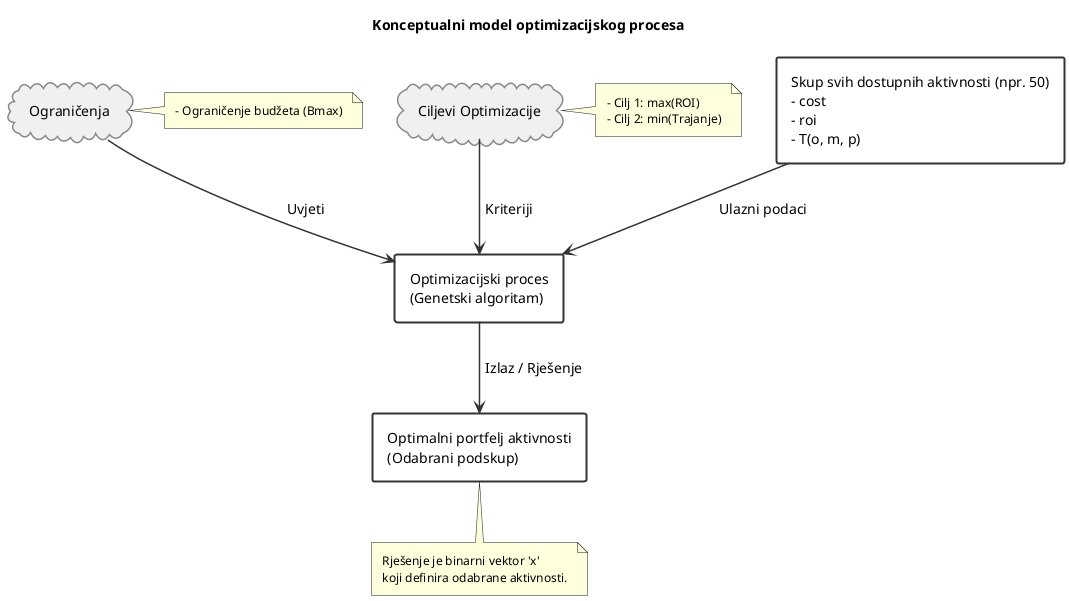
\includegraphics[width=0.8\textwidth]{slike/model_problema.png}
    \caption{Konceptualni model problema optimizacije portfelja projektnih aktivnosti.}
    \label{fig:konceptualni_model}
\end{figure}

Ovaj formalizirani model omogućuje jasnu matematičku i vizualnu reprezentaciju optimizacijskog zadatka. Precizna definicija ulaza, ograničenja i ciljeva ključna je za sustavnu primjenu optimizacijskih metoda poput genetskih algoritama \cite{Mitchell1998} u kombinaciji s Monte Carlo simulacijama \cite{Rubinstein2016}, kako bi se dobila rješenja visoke kvalitete koja su istovremeno i robusna na prisutne nesigurnosti.

\newpage

\section{Zaključak}

U ovom diplomskom radu predstavili smo kompleksan pristup optimizaciji raspodjele projektnih aktivnosti koristeći kombinaciju genetskih algoritama i Monte Carlo simulacije. Cilj je bio razviti model koji uzima u obzir nesigurnost u trajanju, troškovima i vrijednosti zadataka, te u okviru zadanih ograničenja vremena, budžeta i raspoloživih resursa maksimizira ukupnu vrijednost projekta.

Kroz detaljnu analizu problematike i pregled postojeće literature, identificirali smo ključne izazove u upravljanju projektima, posebice u segmentu neizvjesnosti i složenosti optimizacije. Implementacijom metaheurističkih metoda, u ovom slučaju genetskih algoritama \cite{Goldberg1989, Mitchell1998}, omogućili smo efikasno pretraživanje velikog prostora rješenja, dok je Monte Carlo simulacija služila za kvantitativno modeliranje rizika i nesigurnosti \cite{Miller2009, Avlijas2008}, dajući time realističniju procjenu performansi optimizacijskog rješenja.

Praktična implementacija rezultirala je modelom koji omogućuje donošenje informiranih odluka u planiranju i upravljanju projektima, pružajući projektnim menadžerima alate za bolje usklađivanje ciljeva i ograničenja. Pokazalo se da je kombinacija ovih metoda učinkovita u pronalasku balansiranih rješenja koja maksimiziraju povrat ulaganja, uz minimizaciju rizika od prekoračenja budžeta ili rokova.

Iako su postignuti rezultati zadovoljavajući, postoje brojna područja za buduća istraživanja i unaprjeđenja, među kojima izdvajamo:
\begin{itemize}
    \item Proširenje modela na dinamičke uvjete projekata koji se mijenjaju tijekom vremena, uključujući nepredvidive vanjske utjecaje.
    \item Integracija dodatnih metaheurističkih i hibridnih algoritama, poput algoritama rojčaste inteligencije ili simuliranog kaljenja, radi poboljšanja kvalitete rješenja \cite{Gandomi2013}.
    \item Primjena tehnika strojnog učenja za preciznije predviđanje distribucija nesigurnosti i automatsku adaptaciju parametara optimizacije.
    \item Razvoj softverskih alata s intuitivnim korisničkim sučeljem za praktičnu primjenu predloženih metoda u realnim projektnim okruženjima.
\end{itemize}

Zaključno, ovaj rad potvrđuje važnost primjene naprednih algoritamskih rješenja u upravljanju projektima, posebno u uvjetima nesigurnosti, te doprinosi boljem razumijevanju i praktičnoj primjeni optimizacijskih i simulacijskih metoda u području projektne ekonomike i menadžmenta. Kao što ističe Kerzner \cite{Kerzner2017}, učinkovito upravljanje projektima u suvremenom okruženju zahtijeva kombinaciju tradicionalnih i naprednih pristupa, a naš model pruža značajan doprinos u tom smjeru.



\newpage

\bibliographystyle{unsrt}
\bibliography{literatura}
\newpage

%Automatski generira listu svih slika
\listoffigures
\newpage

%Automatski generira listu svih tablica
\listoftables
\newpage


\end{document}
